\chapter{Modes, Jogging and Homing}
\label{ch:modes}

The panel's mode selector decides what the axis keys do and which page the interface puts
in front. The interface never changes the panel's mode and never jogs: it follows.

\begin{notebox}
  Every position on the selector is described in section~\ref{ch:panel}. This chapter
  describes what the operator does in each of them.
\end{notebox}

\section{EDIT, AUTO and MDI}

\begin{description}[font=\normalfont\sffamily\bfseries, leftmargin=2.6cm, style=nextline]
  \item[EDIT] Selects the Program page in the \sbtn{CODE} layout with the editor focused and
        editable. Saving is only possible here.
  \item[AUTO] Brings the Machine page forward. Cycle start is the panel's key; the interface
        shows the line, the progress and the toolpath.
  \item[MDI] Opens the Machine page with the MDI pane in place of the program card. See
        chapter~\ref{ch:mdi}.
\end{description}

Leaving EDIT with an unsaved buffer raises a warning once, because the controller refuses a
save outside EDIT and AUTO can therefore only run the loaded file. The dialog offers
\sbtn{DISCARD BUFFER} and \sbtn{KEEP}.

\section{JOG: continuous jogging}

\begin{itemize}
  \item Hold an axis key on the panel. The axis moves while the key is held.
  \item \pbtn{RAPID} with an axis key moves at rapid rate; the rapid lamp lights.
  \item The jog speed is the profile's \texttt{[jog] max\_speed} (or \texttt{rapid\_speed}
        with RAPID), scaled by the feed override. It is a machine setting, not a screen
        setting.
  \item The Manual page shows the live position, the trail and the loaded program path while
        you jog. It offers no jog buttons.
\end{itemize}

\section{INC: step jogging}

Each key press moves exactly one increment. The increments are the machine INI's
\texttt{[DISPLAY] INCREMENTS} list, so the interface offers exactly the steps the controller
was configured with.

\begin{itemize}
  \item The increment row appears on the Manual page in INC mode.
  \item \keycap{1} to \keycap{9} select the step that carries that number. The list's leading
        \texttt{JOG} entry is continuous jog, which is a mode, and is not offered as a step.
  \item The selection goes to the controller as \halpin{linc.jog-increment} and is remembered
        across sessions.
\end{itemize}

\shot{img/ui/manual-inc.png}{The Manual page in INC mode. The increment row appears under the
coordinates, because the step moves those coordinates.}{fig:manual-inc}

\section{MPG: the handwheel}

MPG enables jogging from the machine's handwheel. Rotate the dial to move the selected axis;
the handwheel's own keys select the axis and the step. The Manual page shows the mode, the
axis selection, the coordinates and the trail.

\begin{notebox}
  The handwheel is a jog input only. Its mode, cycle, spindle, coolant, override, program
  and macro keys are not wired into the interface or the controller's control paths. Outside
  MPG its jog input is ignored as well.
\end{notebox}

\section{Zeroing an axis while setting up}

In JOG, INC, MPG, HOME and PROG.HOME the Manual and Homing pages accept touch-off keys. They
write the work offset; they do not move the machine.

\begin{center}
\begin{tabular}{ll}
  \toprule
  \textbf{Key} & \textbf{Action} \\
  \midrule
  \keycap{X} / \keycap{Y} / \keycap{Z} & Set the active work coordinate of that axis to zero \\
  \keycap{A} & Set every axis to zero \\
  \keycap{O} & Toggle the limit-switch override \\
  \bottomrule
\end{tabular}
\end{center}

The keys are refused when the machine is off, an axis is not homed, the interpreter is busy
or program protect is on. \keycap{A} means something different on other pages; see
chapter~\ref{ch:quickref}.

\section{HOME: homing}

\begin{figure}[H]
  \centering
  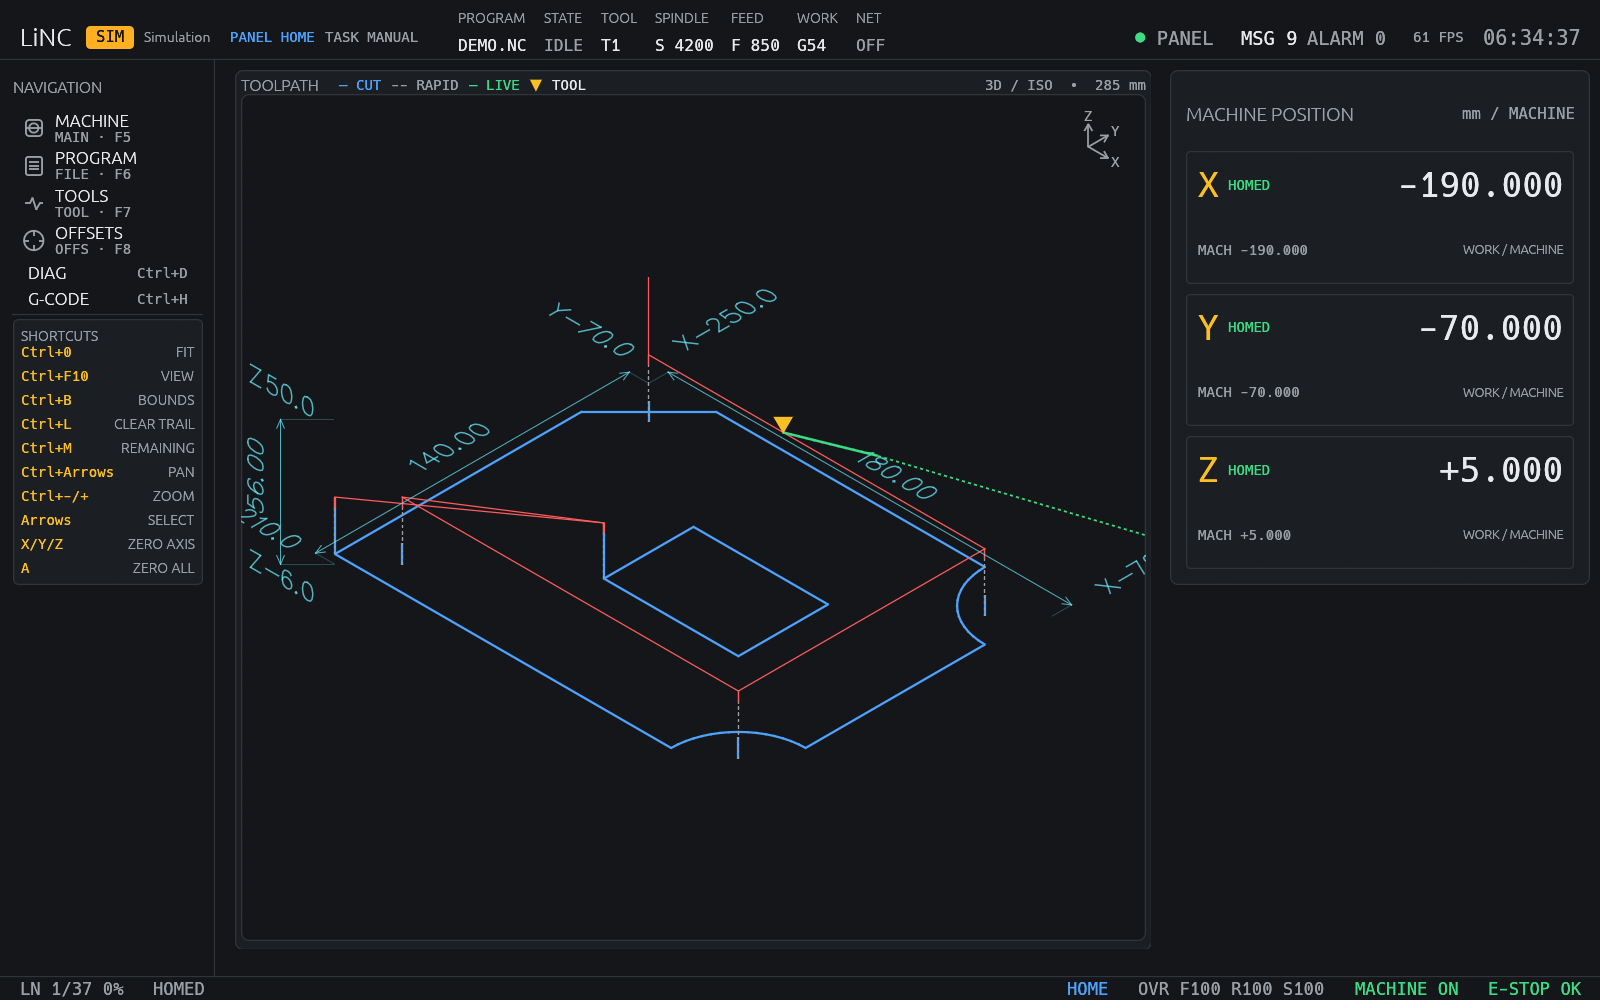
\includegraphics[width=\textwidth]{img/ui/homing.png}
  \caption{The Homing page in HOME mode: machine position with a homing badge per axis, and
           the same toolpath as the Manual page.}
  \label{fig:homing}
\end{figure}

Homing establishes the machine reference. It is required after power-on and after a loss of
reference. Which key homes which axis is the machine's HAL wiring, and the page documents it.

\begin{enumerate}
  \item Turn the selector to \textbf{HOME}. The Homing page opens.
  \item Press \pbtn{RAPID} to home all axes, or the axis key of a single axis.
  \item Each axis row shows a badge: \state{HOMED}, \state{HOMING}, \state{NOT HOMED},
        \state{UNKNOWN} or \state{NOT CONFIGURED}.
  \item The bottom bar changes from \state{NOT HOMED} to \state{HOMED} when every axis is
        home.
\end{enumerate}

The homing order and the search, latch and index settings come from the machine INI and are
shown on the page. With \texttt{NO\_FORCE\_HOMING = 0}, no program and no MDI block runs
before the axes are homed.

\begin{cautionbox}
  Keep a hand near \pbtn{CYCLE STOP} while homing. Check that the table is clear of clamps and
  tools before Z moves.
\end{cautionbox}

\begin{notebox}
  LiNC does not home an axis. The panel's home keys drive the controller's homing input
  directly, which is why homing keeps working when the interface is busy or restarting.
\end{notebox}

\section{PROG.HOME: returning to program zero}

\begin{figure}[H]
  \centering
  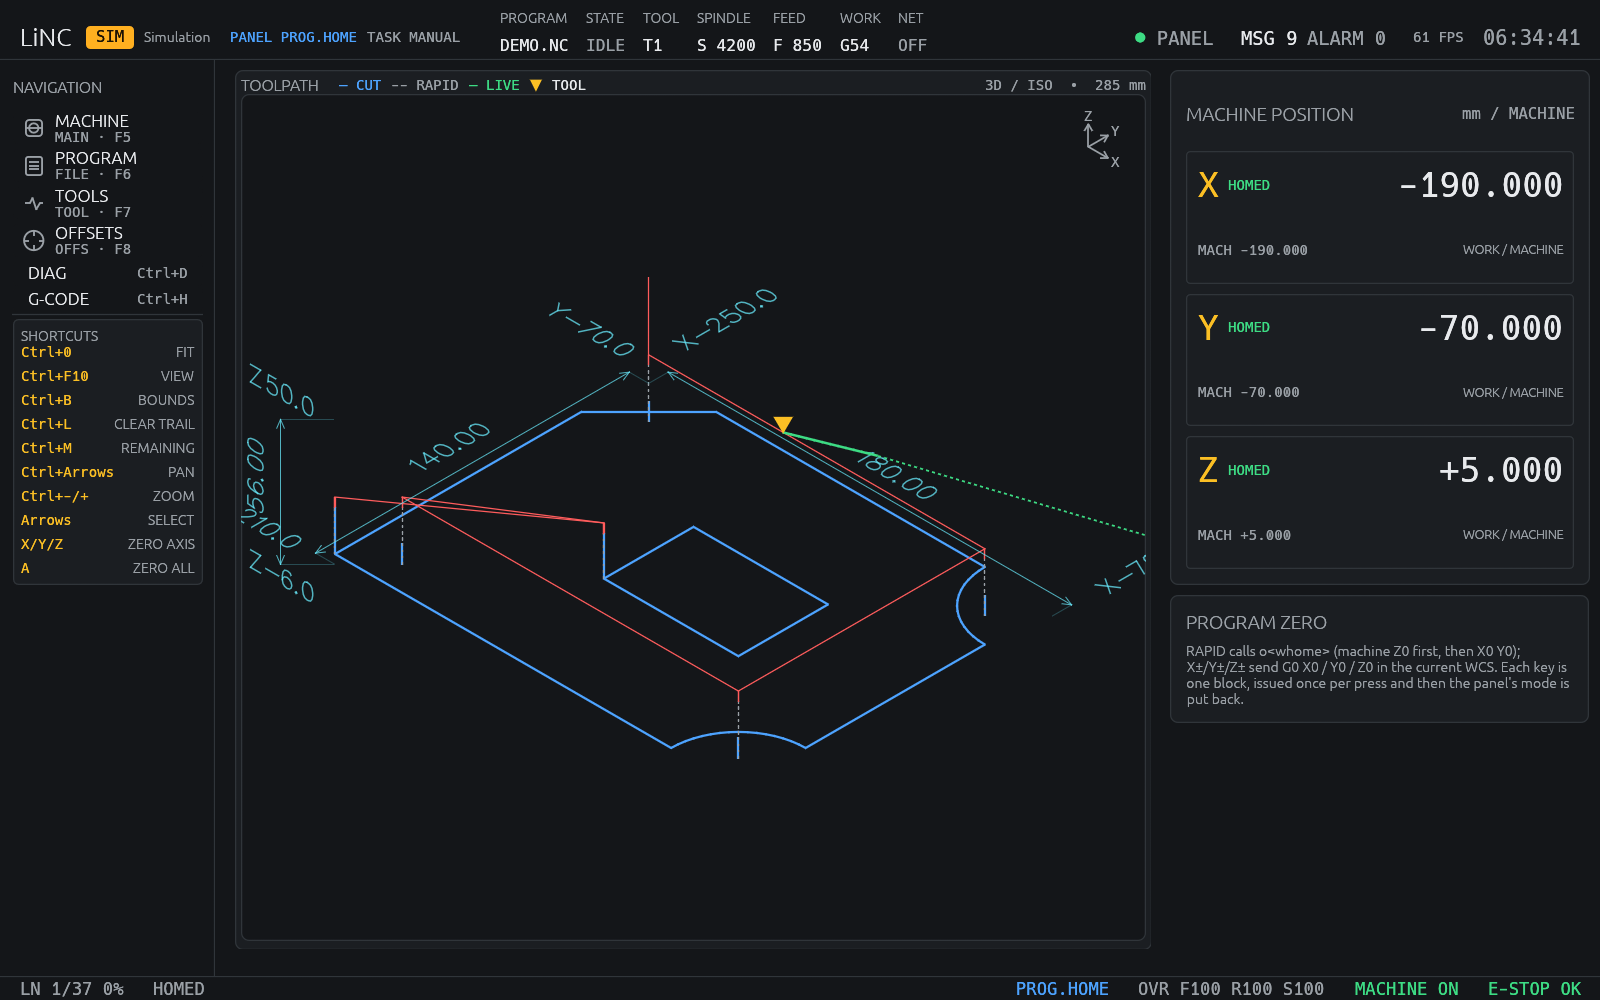
\includegraphics[width=\textwidth]{img/ui/proghome.png}
  \caption{The same page in PROG.HOME mode. The readout is headed \state{PROGRAM ZERO}; the
           panel keys send program-zero blocks.}
  \label{fig:proghome}
\end{figure}

In PROG.HOME the axis keys are not jogs. Each press sends one block, and the interface issues
it:

\begin{center}
\begin{tabular}{ll}
  \toprule
  \textbf{Key} & \textbf{Block} \\
  \midrule
  \pbtn{RAPID} & \texttt{o<whome> call}: machine \texttt{Z0} first, then work \texttt{X0 Y0} \\
  \pbtn{X+} / \pbtn{X-} & \texttt{G0 X0} \\
  \pbtn{Y+} / \pbtn{Y-} & \texttt{G0 Y0} \\
  \pbtn{Z+} / \pbtn{Z-} & \texttt{G0 Z0} \\
  \bottomrule
\end{tabular}
\end{center}

\begin{itemize}
  \item One block per press: a held key does not repeat.
  \item The blocks move to the program zero of the \emph{active} work coordinate system. This
        is not machine home and not \texttt{G53}.
  \item The press is refused, and logged, while the machine is off, an axis is unhomed, the
        interpreter is busy or program protect is on.
  \item The all-axes block lifts Z before it moves X and Y. A single \texttt{G0 X0 Y0 Z0}
        would drag the tool through the part.
\end{itemize}

\section{The Manual page}

\begin{figure}[H]
  \centering
  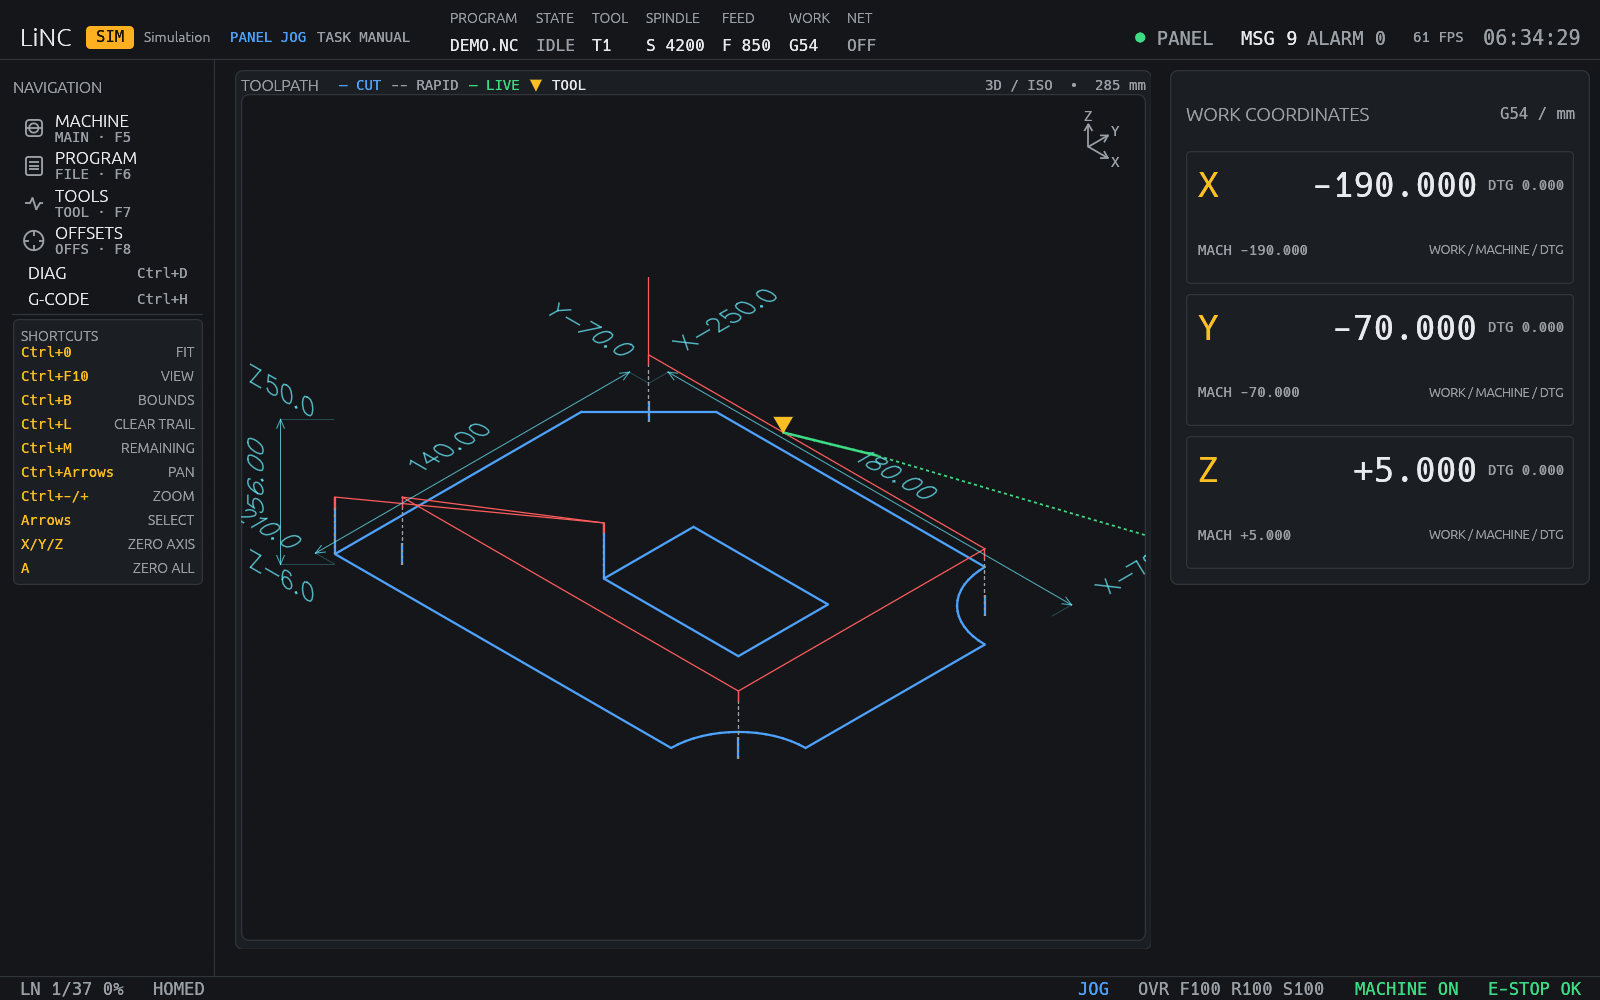
\includegraphics[width=\textwidth]{img/ui/manual.png}
  \caption{The Manual page in JOG mode: toolpath with the loaded program as a muted
           reference, and the work coordinates.}
  \label{fig:manual}
\end{figure}

The Manual page is read-only apart from the increment row and the touch-off keys. It shows:

\begin{itemize}
  \item the toolpath, with the loaded program drawn as a reference and the live trail in its
        own colour;
  \item the work coordinates, the machine coordinates and the distance to go for every axis;
  \item the active axis, highlighted from the panel's axis selection. An unknown selection
        is shown as a dash, never guessed.
\end{itemize}

\begin{tipbox}
  \chordtwo{Ctrl}{0} re-frames the drawing on the tool where it is now. After a long
  jog the trail can drag the view, and a fit brings the part and the tool back together.
\end{tipbox}
